\documentclass{beamer}

\mode<presentation>
{
  \usetheme[hideothersubsections]{MorrisStyle}
  \setbeamercovered{transparent}
}

\usepackage[english]{babel}
\usepackage[latin1]{inputenc}
\usepackage{times}
\usepackage[T1]{fontenc} 
\usepackage{amsmath}

\newcommand{\linespace}{\vskip 0.25cm}

\definecolor{MyForestGreen}{rgb}{0,0.7,0} 
\newcommand{\tableemph}[1]{{#1}}
\newcommand{\tablewin}[1]{\tableemph{#1}}
\newcommand{\tablemid}[1]{\tableemph{#1}}
\newcommand{\tablelose}[1]{\tableemph{#1}}

\definecolor{MyLightGray}{rgb}{0.6,0.6,0.6}
\newcommand{\tabletie}[1]{\color{MyLightGray} {#1}}

% The text in square brackets is the short version of your title and will be used in the
% header/footer depending on your theme.
\title[Energy Optimization Techniques]{Modern Energy Optimization Techniques for a Green Cloud}

% Sub-titles are optional - uncomment and edit the next line if you want one.
% \subtitle{Why does sub-tree crossover work?} 

% The text in square brackets is the short version of your name(s) and will be used in the
% header/footer depending on your theme.
\author[Donatucci]{David Donatucci}

% The text in square brackets is the short version of your institution and will be used in the
% header/footer depending on your theme.
\institute[UMM]
{
  Division of Science and Mathematics \\
  University of Minnesota, Morris \\
  Morris, Minnesota, USA
}

% The text in square brackets is the short version of the date if you need that.
\date[December '14, Senior Seminar] % (optional)
{December 6th 2014 \\ Senior Seminar Conference, Morris, MN}

% Delete this, if you do not want the table of contents to pop up at
% the beginning of each subsection:
\AtBeginSection[]
{
  \begin{frame}<beamer>
    \frametitle{Outline}
    \tableofcontents[currentsection, hideothersubsections]
  \end{frame}
}

\begin{document}

\begin{frame}
  \titlepage
\end{frame}

% For a 20-25 minute senior seminar talk you probably want something like:
% - Two or three major sections (other than the summary).
% - At *most* three subsections per section.
% - Talk about 30s to 2min per frame. So there should probably be between
%   15 and 30 frames, all told.

\section*{Overview}

\subsection*{The Big Picture}

\begin{frame}
  \frametitle{The Big Picture}
  
  \begin{itemize}
	\item Data centers account for a significant fraction of all electricity used in the world.
	\item Large demand for cloud computing means providers must find ways to reduce energy.
	\item High incentive for reduction of energy.
	\item Implementing these techniques may be used to improve data center efficiency.  
  \end{itemize}

  
\end{frame}

\subsection*{Outline}

\begin{frame}
  \frametitle{Outline}
  \tableofcontents[hideallsubsections]
\end{frame}

\section[Cloud Computing]{Cloud Computing Basics}

\subsection{Cloud Computing}

\begin{frame}
  \frametitle{Cloud Computing}
 

\end{frame}

\begin{frame}
  \frametitle{Cloud Computing and Energy}
 

\end{frame}

\subsection{Macro vs Micro Algorithms}

\begin{frame}
  \frametitle{Macro vs Micro}
 

\end{frame}

\section[Green Monster]{Green Monster}
\begin{frame}
  \frametitle{Green Monster}
\begin{columns}
\begin{column}{0.65\textwidth}
  \begin{itemize}
 		\item Evolutionary Multi-Objective Optimization Algorithm (EMOA)
 		\begin{itemize}
 			\item Based upon biological principles.
 			\item Individuals form a population.
 		\end{itemize}
	\item Multiple Optimizations
 		\begin{itemize}
			\item Renewable Energy (RE)
			\item Cooling Energy (CE)
			\item User-to-Service Distance (USD)
		\end{itemize}
	\item Three Steps in EMOA: 
		\begin{itemize}
			\item Initialization
			\item Evolution
			\item Termination
		\end{itemize}
  \end{itemize}
\end{column}
\begin{column}{0.35\textwidth}
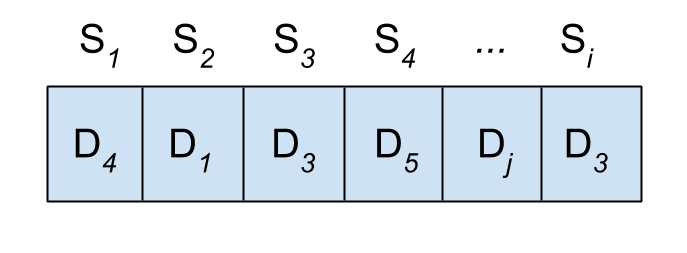
\includegraphics[width=.95\textwidth]{Individual.png} \\
\tiny{Example of an Individual. $S_i$ indicates a service, $D_j$ indicates a data center.}
\end{column}
\end{columns}


\end{frame}
 	
\subsection[Intialization]{EMOA Intialization}

\begin{frame}
\frametitle{EMOA Intialization}
  \begin{itemize}
	\item Individuals length is equivalent to number of services.
	\item Each service is assigned to a random data center. 
	\item Capacity aware randomization.
	\item Creates 100 individuals.
  \end{itemize}
\end{frame}

\subsection[Evolution]{EMOA Evolution}
\begin{frame}
\frametitle{EMOA Evolution}
\begin{columns}
\begin{column}{0.65\textwidth}
  \begin{itemize}
	\item Transformations
		\begin{itemize}
		\item Crossover (90\%)
		\item Mutation (10\%)
		\item Local Search (10\%)
		\item Elitism (N+N)
		\end{itemize}
	\item Transformations occur over 100 Generations.
  \end{itemize}
\end{column}
\begin{column}{0.35\textwidth}
To add: pictures of transformations
%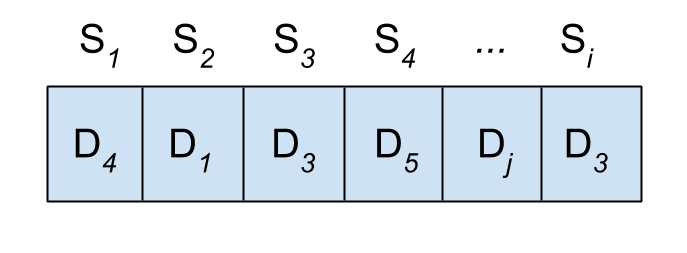
\includegraphics[width=.95\textwidth]{Individual.png} \\
%\tiny{Example of an Individual. $S_i$ indicates a service, $D_j$ indicates a data center.}
\end{column}
\end{columns}
\end{frame}

\subsection[Termination]{EMOA Termination}
\begin{frame}
\frametitle{Evolutionary Multi-Objective Optimization Algorithm (EMOA)}
\begin{columns}
\begin{column}{0.65\textwidth}
  \begin{itemize}
  	\item EMOAs are based upon biological principles.
	\item Individuals form a population.
	\item Multiple Optimizations and Fitness
	\item Transformations
		\begin{itemize}
		\item Crossover
		\item Mutation
		\item Local Search
		\item Elitism
		\end{itemize}
	\item Transformations occur over a specified number of generations.
	\item Individuals that have the lowest fitness are the most optimized to all optimization. 
  \end{itemize}
\end{column}
\begin{column}{0.35\textwidth}
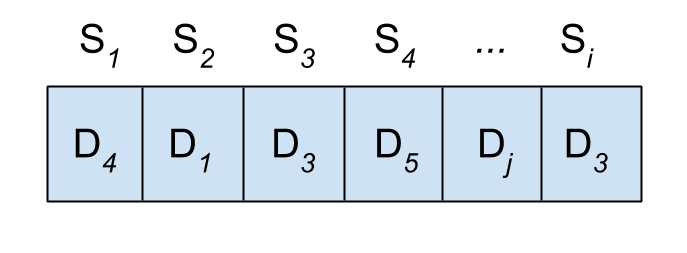
\includegraphics[width=.95\textwidth]{Individual.png} \\
\tiny{Example of an Individual. $S_i$ indicates a service, $D_j$ indicates a data center.}
\end{column}
\end{columns}
\end{frame}

\subsection[Simulations]{Green Monster Simulations}

\begin{frame}
\frametitle{Run Configurations}
\begin{description}[align=left, leftmargin=*]
{\small
\item[Population Initialization] Randomly assigned services to data centers
\item[Optimizations] Maximization of Renewable Energy (RE), Minimization of Cooling Energy (CE) User-to-Service Distance USD
\item[Transform Percentages] crossover (90\%) mutation (10\%)
\item[Local Search Rate] 10\%
\item[Generations] 100
\item[Population Size Per Gen] 1,000 (3 runs) and 10,000 (1 run)
\item[Elitism] N+N\%
}
\end{description}
\end{frame}

\section[GRMP-Q]{Gossip-based Resource Allocation}

\begin{frame}
	\frametitle{Gossip}
	
\end{frame}

\section[Results]{Results}
\subsection{Green Monster}
\subsection{GRMP-Q}

\section[Conclusions]{Conclusions}

\section*{References}

\begin{frame} 
\frametitle{References}
\nocite{*}
\bibliographystyle{acm}
{\tiny \bibliography{annotated_bibliography}}
\end{frame} 

\end{document}